% Template for PLoS
% Version 3.4 January 2017
%
% % % % % % % % % % % % % % % % % % % % % %
%
% -- IMPORTANT NOTE
%
% This template contains comments intended 
% to minimize problems and delays during our production 
% process. Please follow the template instructions
% whenever possible.
%
% % % % % % % % % % % % % % % % % % % % % % % 
%
% Once your paper is accepted for publication, 
% PLEASE REMOVE ALL TRACKED CHANGES in this file 
% and leave only the final text of your manuscript. 
% PLOS recommends the use of latexdiff to track changes during review, as this will help to maintain a clean tex file.
% Visit https://www.ctan.org/pkg/latexdiff?lang=en for info or contact us at latex@plos.org.
%
%
% There are no restrictions on package use within the LaTeX files except that 
% no packages listed in the template may be deleted.
%
% Please do not include colors or graphics in the text.
%
% The manuscript LaTeX source should be contained within a single file (do not use \input, \externaldocument, or similar commands).
%
% % % % % % % % % % % % % % % % % % % % % % %
%
% -- FIGURES AND TABLES
%
% Please include tables/figure captions directly after the paragraph where they are first cited in the text.
%
% DO NOT INCLUDE GRAPHICS IN YOUR MANUSCRIPT
% - Figures should be uploaded separately from your manuscript file. 
% - Figures generated using LaTeX should be extracted and removed from the PDF before submission. 
% - Figures containing multiple panels/subfigures must be combined into one image file before submission.
% For figure citations, please use "Fig" instead of "Figure".
% See http://journals.plos.org/plosone/s/figures for PLOS figure guidelines.
%
% Tables should be cell-based and may not contain:
% - spacing/line breaks within cells to alter layout or alignment
% - do not nest tabular environments (no tabular environments within tabular environments)
% - no graphics or colored text (cell background color/shading OK)
% See http://journals.plos.org/plosone/s/tables for table guidelines.
%
% For tables that exceed the width of the text column, use the adjustwidth environment as illustrated in the example table in text below.
%
% % % % % % % % % % % % % % % % % % % % % % % %
%
% -- EQUATIONS, MATH SYMBOLS, SUBSCRIPTS, AND SUPERSCRIPTS
%
% IMPORTANT
% Below are a few tips to help format your equations and other special characters according to our specifications. For more tips to help reduce the possibility of formatting errors during conversion, please see our LaTeX guidelines at http://journals.plos.org/plosone/s/latex
%
% For inline equations, please be sure to include all portions of an equation in the math environment.  For example, x$^2$ is incorrect; this should be formatted as $x^2$ (or $\mathrm{x}^2$ if the romanized font is desired).
%
% Do not include text that is not math in the math environment. For example, CO2 should be written as CO\textsubscript{2} instead of CO$_2$.
%
% Please add line breaks to long display equations when possible in order to fit size of the column. 
%
% For inline equations, please do not include punctuation (commas, etc) within the math environment unless this is part of the equation.
%
% When adding superscript or subscripts outside of brackets/braces, please group using {}.  For example, change "[U(D,E,\gamma)]^2" to "{[U(D,E,\gamma)]}^2". 
%
% Do not use \cal for caligraphic font.  Instead, use \mathcal{}
%
% % % % % % % % % % % % % % % % % % % % % % % % 
%
% Please contact latex@plos.org with any questions.
%
% % % % % % % % % % % % % % % % % % % % % % % %

\documentclass[10pt,letterpaper]{article}
\usepackage[top=0.85in,left=2.75in,footskip=0.75in]{geometry}

% amsmath and amssymb packages, useful for mathematical formulas and symbols
\usepackage{amsmath,amssymb}

% Use adjustwidth environment to exceed column width (see example table in text)
\usepackage{changepage}

% Use Unicode characters when possible
\usepackage[utf8x]{inputenc}

% textcomp package and marvosym package for additional characters
\usepackage{textcomp,marvosym}

% cite package, to clean up citations in the main text. Do not remove.
\usepackage{cite}

% Use nameref to cite supporting information files (see Supporting Information section for more info)
\usepackage{nameref,hyperref}

% line numbers
\usepackage[right]{lineno}

% ligatures disabled
\usepackage{microtype}
\DisableLigatures[f]{encoding = *, family = * }

% color can be used to apply background shading to table cells only
\usepackage[table]{xcolor}

% array package and thick rules for tables
\usepackage{array}

% create "+" rule type for thick vertical lines
\newcolumntype{+}{!{\vrule width 2pt}}

% create \thickcline for thick horizontal lines of variable length
\newlength\savedwidth
\newcommand\thickcline[1]{%
  \noalign{\global\savedwidth\arrayrulewidth\global\arrayrulewidth 2pt}%
  \cline{#1}%
  \noalign{\vskip\arrayrulewidth}%
  \noalign{\global\arrayrulewidth\savedwidth}%
}

% \thickhline command for thick horizontal lines that span the table
\newcommand\thickhline{\noalign{\global\savedwidth\arrayrulewidth\global\arrayrulewidth 2pt}%
\hline
\noalign{\global\arrayrulewidth\savedwidth}}


% Remove comment for double spacing
\usepackage{setspace} 
\doublespacing

% Text layout
\raggedright
\setlength{\parindent}{0.5cm}
\textwidth 5.25in 
\textheight 8.75in

% Bold the 'Figure #' in the caption and separate it from the title/caption with a period
% Captions will be left justified
\usepackage[aboveskip=1pt,labelfont=bf,labelsep=period,justification=raggedright,singlelinecheck=off]{caption}
\renewcommand{\figurename}{Fig}

% Use the PLoS provided BiBTeX style
\bibliographystyle{plos2015}

% Remove brackets from numbering in List of References
\makeatletter
\renewcommand{\@biblabel}[1]{\quad#1.}
\makeatother

% Leave date blank
\date{}

% Header and Footer with logo
\usepackage{lastpage,fancyhdr,graphicx}
\usepackage{epstopdf}
\pagestyle{myheadings}
\pagestyle{fancy}
\fancyhf{}
\setlength{\headheight}{27.023pt}
\lhead{\includegraphics[width=2.0in]{PLOS-submission.eps}}
\rfoot{\thepage/\pageref{LastPage}}
\renewcommand{\footrule}{\hrule height 2pt \vspace{2mm}}
\fancyheadoffset[L]{2.25in}
\fancyfootoffset[L]{2.25in}
\lfoot{\sf PLOS}

%% Include all macros below

\newcommand{\suppfigsimpleaccess}{1}
\newcommand{\suppfigsparseschem}{2}
\newcommand{\suppfigsparsecol}{3}
\newcommand{\suppfigsparserow}{4}
\newcommand{\suppfighdfspeed}{5}
\newcommand{\suppfighdflayout}{6}
\newcommand{\suppfighdfrandom}{7}

\newcommand{\suppsecsimdesign}{1.1}
\newcommand{\suppsecsimple}{1.2}
\newcommand{\suppsecsparse}{1.3}
\newcommand{\suppsechdfmat}{1.4}
\newcommand{\suppsecother}{1.5}
\newcommand{\suppseclayoutoptim}{2}
\newcommand{\suppseclayoutrandom}{3}
\newcommand{\suppsecrealzeisel}{4.1}
\newcommand{\suppsecrealtenx}{4.2}

\newcommand{\beachmat}{\textit{beachmat}}
\newcommand{\code}[1]{\texttt{#1}}
\newcommand{\revised}[1]{\textcolor{red}{#1}}

%% END MACROS SECTION

% Other required things:
\usepackage{subcaption}
\captionsetup[subfigure]{justification=centering}

% document begins here
\begin{document}

% Title must be 250 characters or less.
\begin{flushleft}
{\Large
\textbf\newline{beachmat: a Bioconductor C++ API for accessing single-cell genomics data from a variety of R matrix types} % Please use "sentence case" for title and headings (capitalize only the first word in a title (or heading), the first word in a subtitle (or subheading), and any proper nouns).
}
\newline
% Insert author names, affiliations and corresponding author email (do not include titles, positions, or degrees).
\\

Aaron T. L. Lun\textsuperscript{1*},
Herv\'e Pag\`es\textsuperscript{2},
Mike L. Smith\textsuperscript{3}
\\
\bigskip
\textbf{1} Cancer Research UK Cambridge Institute, University of Cambridge, Li Ka Shing Centre, Robinson Way, Cambridge CB2 0RE, United Kingdom 
\\
\textbf{2} Fred Hutchinson Cancer Research Center, 1100 Fairview Ave N, Seattle, WA 98109, USA
 \\
\textbf{3} European Molecular Biology Laboratory (EMBL), Genome Biology Unit, 69117 Heidelberg, Germany
\\
\bigskip

% Insert additional author notes using the symbols described below. Insert symbol callouts after author names as necessary.

% Use the asterisk to denote corresponding authorship and provide email address in note below.
* aaron.lun@cruk.cam.ac.uk

\end{flushleft}
% Please keep the abstract below 300 words
\section*{Abstract}
Recent advances in single-cell RNA sequencing (scRNA-seq) have dramatically increased the number of cells that can be profiled in a single experiment.
This provides unparalleled resolution to study cellular heterogeneity within biological processes such as differentiation.
However, the explosion of data that are generated from such experiments poses a challenge to the existing computational infrastructure for statistical data analysis.
In particular, large matrices holding expression values for each gene in each cell require sparse or file-backed representations for manipulation with the popular R programming language.
These alternative representations are not easily compatible with high-performance C++ code used for computationally intensive tasks in existing R packages.
Here, we describe a C++ interface named \beachmat{}, which enables agnostic data access from various matrix representations.
This allows package developers to write efficient C++ code that is interoperable with simple, sparse and file-backed matrices, amongst others.
We evaluated the performance of \beachmat{} on each matrix representation using both simulated and real scRNA-seq data, and defined a clear memory/speed trade-off to motivate the choice of an appropriate representation.
We also demonstrate how beachmat can be incorporated into the code of other packages to drive analyses of a very large scRNA-seq data set.

\linenumbers

\section*{Introduction}
Recent advances in single-cell RNA sequencing (scRNA-seq) technologies have led to an explosion in the quantity of data that can be generated in routine experiments.
Droplet-based methods such as Drop-Seq \cite{macosko2015highly}, inDrop \cite{klein2015droplet} and GemCode \cite{zheng2017massively} allow transcriptome-wide expression profiles involving 10,000-40,000 genes to be captured in each of thousands to millions of cells.
Careful computational analysis is critical to extract meaningful biology from these data, but their sheer volume strains existing pipelines and methods designed for single-cell data processing.
The data analysis challenge is compounded by the presence of large-scale projects such as the Human Cell Atlas \cite{regev2017human}, which aims to use single-cell `omics to profile every cell type in the human body.
Similar issues are encountered outside of transcriptomics, with single-cell ATAC-seq \cite{buenrostro2015single} and bisulfite sequencing \cite{smallwood2014single} providing region- to base-level resolution of biochemical events (chromatin accessibility and DNA methylation, respectively).

The statistical programming language R \cite{R} is a key platform for processing and exploring scRNA-seq data sets.
R provides efficient, rigorously tested, open-source implementations of many statistical and numerical procedures.
Its interactive nature lends itself to data exploration and research, while its programming features allow assembly of complex analyses.
It is also extensible through the installation of optional ``packages", often contributed by the research community, which contain bespoke methods for specific scientific problems.
In particular, the Bioconductor project \cite{gentleman2004bioconductor,huber2015orchestrating} provides packages for biological data analysis, many of which implement established methods for single-cell `omics data analysis \cite{trapnell2014dynamics,lun2016pooling,mccarthy2017scater,finak2015mast}
Packages are mostly written in R but can also include native code (in C/C++ or Fortran) for computationally intensive tasks.
Use of native C++ code is facilitated by the \textit{Rcpp} package \cite{eddelbuettel2011seamless}, which simplifies the integration of package code with the R application programming interface (API).

In its simplest form, a scRNA-seq data set consists of a matrix where each column is a cell, each row is a gene, and the value of each matrix entry is set to the quantified expression (e.g., number of mapped reads, transcripts-per-million) for that gene in that cell.
This is most directly represented in R as a simple matrix, where each entry is explicitly stored in \revised{random access} memory \revised{(RAM)} in a dense contiguous array.
Alternatively, it can be represented as a sparse matrix using classes from the \textit{Matrix} package \cite{bates2017matrix}, which saves memory by only storing non-zero entries.
This exploits the low capture efficiencies of current scRNA-seq protocols \cite{grun2015design} that are responsible for the high frequency of zeroes in the data.
Another option is to use file-backed representations such as those in the \textit{bigmemory} \cite{kane2013scalable} or \textit{HDF5Array} packages, where the data are stored in \revised{a file} and parts of it are loaded into \revised{RAM} upon request.
In each case, methods are provided in R for common operations such as subsetting, transposition and arithmetic, such that any downstream code for data processing can be agnostic to the exact representation of the matrix.
This simplifies software development and improves interoperability.

Unfortunately, \revised{using alternative matrix representations is less straightforward for} compiled code written in statically typed languages like C++.
\revised{Existing interfaces for passing R matrices into C/C++ require the details of the matrix representation to be specified during compilation.}
This makes it difficult to write a single, general piece of code that can be applied to many different representations.
Writing multiple versions for different representations is difficult and unsustainable when more representations become available.
The alternative is to perform all processing in R to exploit the availability of common methods.
However, this is an unappealing option for high-performance code.
R is often slower than C++ by at least an order of magnitude for arbitrary programming tasks that cannot be ``vectorized'', i.e., made to operate on all elements of a vector at once.
This includes common procedures in scRNA-seq data analysis such as looping across all cells or genes and performing arbitrarily complex operations on the cell- or gene-specific expression profiles.
The use of R alone would increase the computational time required to perform analyses, which is inconvenient for small scripts, undesirable for interactive analyses and unacceptable for large simulation studies.
It would clearly be preferable to implement critical functions (including loops) in native code wherever possible.

% One might think to simply move the inside of the loop in C++ to migitate the interpretation cost, while keeping the loop at the R level to access row- or column-level data.
% However, this involves some costs on its own, e.g., memory allocations that were previously one-offs need to be re-performed.
% If you need to share data across iterations, it will also involve more function calls to store relevant variables, so the cost of function calls is not avoided.

Here, we describe a C++ API named \beachmat{} (using Bioconductor to handle Each Matrix Type), which enables access to R matrix data in a manner that is agnostic to the exact matrix representation.
This allows developers to implement computationally intensive algorithms in C++ that can be immediately applied to a wide range of R matrix classes, including simple matrices, sparse matrices from the \textit{Matrix} package, and HDF5-backed matrices from the \textit{HDF5Array} package.
Using simulated and real scRNA-seq data, we assess the performance of \beachmat{} for data access from each matrix representation.
We show that each representation has specific strengths and weaknesses, with a clear memory-speed trade-off that motivates the use of different representations in different settings.
We also demonstrate how \beachmat{} can be used by other Bioconductor packages to empower the analysis of a very large scRNA-seq data set. 
By operating synergistically with existing Bioconductor infrastructure, \beachmat{} extends R's capabilities for analyzing scRNA-seq and other large matrix data.

\section*{Design and implementation}
The \beachmat{} API uses C++ classes to provide a common interface for data access from R matrix representations.
We define a base class that implements common methods for all representations \revised{of a given data type (e.g., integer, double-precision)}.
Each specific representation is associated with a derived C++ class that provides customized implementations of the access methods.
The intention is for a user to pass in an R matrix of any type, in the form of an \code{RObject} instance from the \textit{Rcpp} API (Figure~\ref{fig:beachoverview}).
\beachmat{} then produces a corresponding C++ object, returning a pointer to the base class.
This pointer is the same regardless of the representation and can be used in downstream C++ code to achieve run-time polymorphism.

\begin{figure}[btp]
    \begin{center}
        \includegraphics[width=\textwidth]{pics/overview.pdf}
    \end{center}
    \caption{Schematic of the \beachmat{} workflow.
        Various matrix representations at the R level are passed as \code{RObject} instances to a C++ function.
        \beachmat{} identifies the specific representation, constructs an instance of the appropriate C++ derived class, and returns a pointer to base class.
        (In this case, a \code{numeric\_matrix} pointer is returned for input matrices holding double-precision data.)
        This pointer can then be used in user-level code in a manner that is agnostic to the details of the original representation.
    }
    \label{fig:beachoverview}
\end{figure}

Access to matrix data is achieved with common methods in the base class that have specialized implementations in each derived class. 
When access to a specific row or column (or a \revised{part} thereof) is requested, the \beachmat{} API will fill a \textit{Rcpp}-style \code{Vector} object with corresponding data values from the matrix.
This strategy provides the greatest flexibility for downstream applications, by allowing in-place modifications to vector elements and guaranteeing contiguous data storage. 
In addition, a request for a specific entry of the matrix will directly return the corresponding data value.

While the \beachmat{} API is agnostic to the matrix representation, it still needs to know the type of data that are stored in the matrix.
We use C++ templating to recycle the code to define specific classes for common data types, i.e., logical, integer, double-precision floating point or character strings.
The same methods are available for all classes of each data type, improving their ease of use for developers.

Currently, \beachmat{} supports data access from a number of widely used matrix representations.
Using simulated data, we measured the speed of data access from each representation with \beachmat{} (Supplementary Section~\suppsecsimdesign{}).
This includes:
\begin{itemize}
    \item Simple R matrices, constructed with the base \texttt{matrix} function or using the \texttt{dgeMatrix} class from the \textit{Matrix} package.
        Here, data are stored in \revised{RAM} as a contiguous dense array in column-major format.
        We demonstrate that \beachmat{} provides comparable performance to a reference \textit{Rcpp} implementation for accessing data from these matrices 
        (Supplementary Section~\suppsecsimple{}, Supplementary Figure~\suppfigsimpleaccess{}). 
    \item Sparse matrices in compressed sparse column-orientated format (Supplementary Section~\suppsecsparse{}, Supplementary Figure~\suppfigsparseschem{}), 
        implemented in the \texttt{dgCMatrix} class from \textit{Matrix}.
        This representation only stores non-zero values in \revised{RAM}, which is highly efficient for single-cell genomics data with many dropouts.
        However, the more complex format means that data access from sparse matrices is generally slower than simple matrices (Supplementary Figure~\suppfigsparsecol{}).
        We use a novel caching strategy to improve the efficiency of accessing data from consecutive rows by avoiding unnecessary binary searches (Supplementary Figure~\suppfigsparserow{}).
        We also show that \beachmat{} provides faster row-level data access than the \textit{RcppArmadillo} API \cite{eddelbuettel2014arma}.
    \item File-backed matrices using the hierarchical data format (HDF5) \cite{hdf5}, 
        implemented in the \texttt{HDF5Matrix} class from the \textit{HDF5Array} package (Supplementary Section~\suppsechdfmat{}).
        This stores the entire data set in a HDF5 file, only retrieving subsets into \revised{RAM} upon request.
        As a result, it is very memory-efficient but much slower than the other representations (Supplementary Figure~\suppfighdfspeed{}).
        A key determinant of access speed is the layout of the HDF5 file, where data can be split into ``chunks'' for easier retrieval.
        Once read, chunks are typically cached in memory to avoid redundant retrieval of data from the same chunk in adjacent rows or columns.
        To improve performance, \beachmat{} automatically tunes the parameters of the HDF5 chunk cache to optimize data access from consecutive rows or columns (Supplementary Figure~\suppfighdflayout{}, Supplementary Section~\suppseclayoutoptim{}).
        We provide functions to choose suitable chunk dimensions during file creation, when consecutive row or column access is expected downstream;
        as well as functions to convert to file layouts that are optimal for random row or column access (Supplementary Figure~\suppfighdfrandom{}, Supplementary Section~\suppseclayoutrandom{}).
\end{itemize}
Other representations are also supported, including packed symmetric matrices and matrices based on run-length encodings (see Supplementary Section~\suppsecother{} for details).
As a general rule, matrix representations that occupy more \revised{RAM} provide faster data access, as data do not need to be unpacked or retrieved from \revised{file}.
\revised{(In practice, the magnitude of differences in access speed between representations depends on many factors such as the amount of microprocessor cache memory, speed of reading data from files on different storage media, etc., which are not considered here.)}

In addition to accessing data in existing matrices, the \beachmat{} API allows C++ code to store data in various representations for output to R.
For integer, logical, double-precision and character data, simple and HDF5-backed matrices can be constructed that are indistinguishable from those generated in R.
Logical and double-precision data can also be stored in sparse format, where only true or non-zero values are retained in \code{lgCMatrix} or \code{dgCMatrix} instances, respectively.
(The \textit{Matrix} package does not support sparse integer or character matrices, so these are not considered.)
The output representation can either be explicitly specified in the code, or it can be automatically chosen to match some input representation.
To illustrate, consider a C++ function that accepts a matrix as input and returns a matrix of similar dimensions.
If the input is in the simple matrix format, one might assume that there is enough RAM to also store the output in the simple format;
whereas if the input is a \code{HDF5Matrix}, one could presume that the output would be similarly large, thus requiring a \code{HDF5Matrix} representation for the results.
This means that results of processing in C++ can be returned in the most suitable representation for manipulation in R.
 
%Note that the layout considerations described for read access to HDF5-backed input are equally applicable to HDF5-backed output.
%If rows/columns are to be filled consecutively, we suggest using rectangular chunks that are proportional to the dimensions of the matrix (Supplementary Section~\suppseclayoutoptim{}).
%For random write access, pure column- or row-based chunks are more suitable.
%Chunk dimensions can be specified directly with the \textit{beachmat} API; or by using functions from the \textit{HDF5Array} package to set the global chunking dimensions in R, which will be respected by \beachmat{} in the C++ code.

We note that an alternative to using \beachmat{} is to write C++ code for simple matrices and apply it to submatrices (or ``blocks'') of a given input matrix.
Each block is coerced to a simple matrix before it is supplied to the C++ code.
After looping across all blocks, the block-wise results are combined to obtain the final result for the entire matrix.
This block processing strategy allows the application of C++ code while controlling RAM usage by storing only one block as a simple matrix at any given time.
However, it requires coordination between R and C++ to keep track of the block that is being processed, to monitor intermediate variables that persist between blocks, and to combine the results in an appropriate manner.
The need to ensure that R and C++ are interacting correctly at multiple points imposes a significant burden on the developer.
Computational efficiency is also reduced by looping in R, multiple matrix coercions and repeated C++ function calls.
The \beachmat{} API provides a natural solution by moving the entire procedure into C++, simplifying development and maintenance.

\section*{Results}

\subsection*{Access times for a small brain data set}
We evaluated the performance of \beachmat{} with the different matrix representations on real scRNA-seq data from a study of the mouse brain by Zeisel \textit{et al.} \cite{zeisel2015brain} (Supplementary Section~\suppsecrealzeisel{}). 
This data set contains integer expression values for 19972 genes in each of 3005 brain cells, derived from different regions of the brain and consisting of a diverse range of cell types.
Only 18\% of expression values in the matrix are non-zero.
The Zeisel \textit{et al.} data set is not particularly large, especially in the context of droplet-based experiments that routinely generate transcriptome-wide data for tens of thousands of cells.
However, for our purposes, the smaller number of cells in this data set is desirable as it means that each of the matrix representations -- including those that are stored \revised{wholly in RAM} -- can be easily evaluated and compared.

We converted the Zeisel \textit{et al.} data to the various matrix representations and measured the access speed for the row- or column-level data with \beachmat{}.
We observed similar results to those obtained with simulated data, recapitulating the different trade-offs between \revised{access} speed and \revised{RAM} usage across representations.
Specifically, row and column accesses from a simple matrix were fastest, followed by accesses from a sparse matrix (Figure~\ref{fig:zeisel}).
HDF5-backed matrices provided slowest access but also the smallest memory footprint (2 KB, compared to 480 MB for simple matrices and 130 MB for sparse matrices).
The size of the HDF5 file was also relatively small, requiring only 16-20 MB of space for each \code{HDF5Matrix} instance.

\begin{figure}[bt]
    \begin{subfigure}[b]{0.49\textwidth}
        \includegraphics[width=\textwidth]{../real/zeisel/pics/zeisel_col.pdf}
        \caption{}
    \end{subfigure}
    \begin{subfigure}[b]{0.49\textwidth}
        \includegraphics[width=\textwidth]{../real/zeisel/pics/zeisel_row.pdf}
        \caption{}
    \end{subfigure}
    \caption{Access times for various matrix representations of the mouse brain data set from Zeisel \textit{et al.} \cite{zeisel2015brain}.
        (a) \revised{Time required to calculate the column sums for each representation by accessing data from each column.}
        For \code{HDF5Matrix}, a column-chunked layout and a rectangular $200 \times 200$ layout were tested.
        (b) \revised{Time required to calculate the row sums for each representation by accessing data from each row.}
        For \code{HDF5Matrix}, a row-chunked layout and a rectangular $200 \times 200$ layout were tested.
        Heights represent the average of 10 repeated timings; standard errors were negligible and not shown.
    }
    \label{fig:zeisel}
\end{figure}

An appropriate choice of matrix representation depends on the context in which it is used.
We could use purely in-\revised{RAM} representations for optimal access speed, but this may not be practical for very large data sets.
Even high-performance computing systems have their limits, especially in academic environments with many users where high-resource jobs are difficult to schedule.
Sparse representations also become ineffective if sparsity-destroying operations (e.g., mean-centering, batch correction) are applied.
In such cases, it may be preferable to sacrifice speed for reduced memory consumption by using file-backed representations such as \code{HDF5Matrix}.
By incorporating \beachmat{} into the C++ code, an R package can dynamically accept different matrix types appropriate for the size of the data set and computing environment.

\subsection*{Analysis of the large 10X data set}
To demonstrate the utility of \beachmat{} for faciliting analyses of large data sets, we converted several functions in the \textit{scater} \cite{mccarthy2017scater} and \textit{scran} packges \cite{lun2016stepbystep} to use \beachmat{} in their C++ code.
We applied these functions to the 1.3 million brain cell data set from 10X Genomics (Supplementary Section~\suppsecrealtenx{}).
First, we called cell cycle phase with the \code{cyclone} method \cite{scialdone2015computational}. 
Most cells were identified as being in G1 phase (Figure~\ref{fig:tenx}a), consistent with the presence of differentiated neurons that are not actively cycling.
Next, we applied the deconvolution method \cite{lun2016pooling} to compute size factors to normalize for cell-specific biases.
The size factor for each cell was generally well-correlated with the library size (Figure~\ref{fig:tenx}b).
However, a few cells have size factors that are much smaller than expected based on their library sizes, and there is a modest amount of scatter around the size factor-library size trend.
This is consistent with composition effects \cite{robinson2010scaling} caused by differential gene expression between cell subpopulations.

\begin{figure}
    \begin{subfigure}[b]{0.49\textwidth}
        \includegraphics[height=2.5in,trim=0mm 0mm 5mm 10mm,clip]{../real/10X/pics/cycle.png}
        \caption{}
    \end{subfigure}
    \begin{subfigure}[b]{0.49\textwidth}
        \includegraphics[height=2.5in,trim=0mm 0mm 5mm 10mm,clip]{../real/10X/pics/sizefacs.png}
        \caption{}
    \end{subfigure}
    \begin{subfigure}[b]{0.49\textwidth}
        \includegraphics[height=2.5in,trim=0mm 0mm 5mm 10mm,clip]{../real/10X/pics/hvg.png}
        \caption{}
    \end{subfigure}
    \begin{subfigure}[b]{0.49\textwidth}
        \includegraphics[height=2.5in,trim=0mm 0mm 5mm 10mm,clip]{../real/10X/pics/pca.png}
        \caption{}
    \end{subfigure}
    \caption{Analysis of the 10X 1.3 million brain cell data set.
        (a) Cell cycle phase assignment, based on the G1 and G2M scores reported by \code{cyclone}.
        The intensity of colour is proportional to the density of cells at each plot location.
        Dashed lines indicate the score boundaries corresponding to each phase, and the number of assigned cells is also shown for each phase.
        (b) Size factor for each cell from the deconvolution method, plotted against the library size.
        Cells were coloured according to the deviation from the median log-ratio of the size factor to the library size for all cells.
        (c) Variance of the normalized log-expression values for each gene, plotted against the mean log-expression.
        The red line indicates the mean-dependent trend fitted to all genes.
        Orange points correspond to highly variable genes detected at a false discovery rate of 5\%, with the top 10 genes highlighted.
        (d) PCA plot generated from the HVG expression profiles of all cells.
        The variance explained by each of the first two principal components is shown in brackets.
    }
    \label{fig:tenx}
\end{figure}

We detected highly variable genes (HVGs) based on the variance of the log-normalized expression values \cite{lun2016stepbystep}.
This was performed while blocking on the sequencing library of origin for each cell, to regress out technical factors of variation unrelated to biological heterogeneity.
We identified a number of HVGs (Figure~\ref{fig:tenx}c), including genes involved in neuronal differentiation and function such as \textit{Neurod6} \cite{ kay2011neurod6} and \textit{Sox11} \cite{bergsland2006establishment}. 
Finally, we performed dimensionality reduction on the HVG expression profiles for all cells using randomized principal components analysis (PCA) \cite{halko2011finding}.
Visualization of the first two principal components (PCs) showed clear substructure in the cell population (Figure~\ref{fig:tenx}d), reflecting the diversity of cell types in the mouse brain.
Indeed, once PCA has been performed, the first 10-100 PCs for each cell can be used as a summary of its expression profile.
This can be stored as a simple matrix and supplied directly to other R functions for clustering \cite{xu2015identification,csardi2006igraph} or trajectory reconstruction \cite{trapnell2014dynamics}.
At this point, memory usage ceases to be an issue for scRNA-seq data analysis, and we only need to choose algorithms that are scalable with respect to the number of cells.

While a full characterisation of this data set is outside the scope of this article, it is clear that we can proceed through many parts of the scRNA-seq analysis pipeline using \beachmat{}-driven C++ functions.
By taking advantage of the file-backed \code{HDF5Matrix}, this analysis can be conducted in reasonable time on a desktop with modest specifications (see Methods).
These features allow us to obtain biological insights that previously would have been inaccessible from R.
We also note that the incorporation of the \beachmat{} API only required small modifications to existing C++ code for scRNA-seq data analysis.
This indicates that many established methods in the R/Bioconductor ecosystem can be easily and immediately extended to work with large data sets,
enabling the statistically rigorous analysis of big single-cell data.

\section*{Availability and future directions}
The \beachmat{} package contains the C++ API and is available as part of version 3.6 of the Bioconductor project (\url{https://bioconductor.org/packages/beachmat}).
It is straightforward to integrate \beachmat{} into existing R packages, enabling arbitrary C++ code to accept many different matrix inputs without any further effort on the part of the developer.
Our modifications to the \textit{scran} and \textit{scater} packages have enabled the analysis of a very large scRNA-seq data set in low-memory environments using file-backed representations, without significantly compromising speed for smaller data sets that can be held fully in memory.
These modifications are now implemented in the latest versions of \textit{scran} and \textit{scater}, both of which can also be installed from Bioconductor.

The popularity of the R programming language stems, in part, from the ease with which it can be extended.
Packages can be easily developed by the research community to implement cutting-edge algorithms for new data types.
The increasing number of packages designed to analyze scRNA-seq data (13 on Bioconductor at time of writing) provides a case in point.
We anticipate that \beachmat{} will be useful to developers of novel computationally intensive bioinformatics methods that need to access data from different matrices.
While we have focused on scRNA-seq in this paper, analyses of other large matrices (e.g., genome-wide contact matrices in Hi-C data \cite{lun2016infrastructure}) may also benefit from \beachmat{}-driven code.
We will also continue to develop \beachmat{} to support data access from new formats such as Loom for scRNA-seq data (\url{http://loompy.org/}).

We note that, for big single-cell data, the utility of \beachmat{} for R package development ultimately depends on the scalability of the underlying algorithms for processing millions or even billions of cells.
Most existing methods for scRNA-seq data analysis are designed to handle thousands of cells at best.
Fortunately, we can make use of the existing expertise in the Bioconductor community to improve scalability.
Highly multiplexed flow and mass cytometry experiments routinely generate low-dimensional data for millions of cells,
and many Bioconductor packages are already available to analyze and interpret these data \cite{finak2014opencyto,weber2016comparison,lun2017testing}.
A low-rank representation of scRNA-seq data (e.g., after PCA) is similar to cytometric data in size and structure, suggesting that algorithms used in the latter can also be applied to the former.
This presents an interesting avenue for future development of software based on \beachmat{}.

All R/C++ code used to perform the simulations and real data analyses are also available on Github (\url{https://github.com/LTLA/MatrixEval2017}).

\section*{Author contributions}
ATLL conceived and implemented the \beachmat{} C++ API, performed the data access simulations and analyzed the 10X data set.
HP adapted the \textit{HDF5Array} and \textit{DelayedArray} packages to interface with \beachmat{}.
MLS ported the HDF5 C++ API into \textit{Rhdf5lib}, to support HDF5 read/write access in \beachmat{}.

\section*{Acknowledgements}
We thank Martin Morgan, Andrew McDavid, Peter Hickey, Raphael Gottardo, Mike Jiang, Vince Carey, John Readey and other members of the Bioconductor single-cell big data working group for useful discussions.
We thank Davis McCarthy for his assistance with incorporating \beachmat{} into \textit{scater}.
We also thank John Marioni for helpful comments on the manuscript.

\section*{Funding statement}
ATLL was supported by core funding from Cancer Research UK (award no. 17197 to Dr.\ John Marioni), the University of Cambridge and Hutchison Whampoa Ltd.
MLS was funded by The German Network for Bioinformatics Infrastructure (de.NBI) F\"orderkennzeichen Nr.\ 031A537 A.

\bibliography{ref}

\end{document}
